\documentclass[sigconf,anonymous]{aamas}
\usepackage{balance}
\usepackage{colortbl}
\usepackage{tabularx}
\usepackage{algorithm}
\usepackage[noend]{algpseudocode}
\usepackage[most]{tcolorbox}
\usepackage{tikz}
\usetikzlibrary{arrows.meta,positioning,shapes.geometric,fit,calc,decorations.pathreplacing}
\graphicspath{{vendor/}}
\setlength{\emergencystretch}{2em}

% Shared visual palette sampled from the reference charts.
\definecolor{degroblue}{HTML}{3D6EAC}
\definecolor{degrogreen}{HTML}{2CC55E}
\definecolor{degroorange}{HTML}{F1AE45}
\definecolor{degrolight}{HTML}{EFEEFF}
\definecolor{degrogray}{HTML}{535353}
\definecolor{degrotableblue}{HTML}{E0DFFF}

\newtcolorbox{takeawaybox}{
  enhanced,
  colback=degrolight,
  colframe=degrogray,
  coltitle=black,
  fonttitle=\bfseries\small,
  colbacktitle=degrogray,
  coltitle=white,
  title=Takeaway,
  fonttitle=\bfseries\small,
  fontupper=\bfseries\normalsize,
  boxrule=0.8pt,
  arc=3pt,
  outer arc=3pt,
  left=7pt,
  right=7pt,
  top=6pt,
  bottom=6pt,
  toptitle=4pt,
  bottomtitle=4pt,
  before skip=6pt,
  after skip=7pt
}
\newcommand{\takeaway}[1]{\begin{takeawaybox}#1\end{takeawaybox}}

\makeatletter
\gdef\@copyrightpermission{%
  \begin{minipage}{0.2\columnwidth}
  \href{https://creativecommons.org/licenses/by/4.0/}{
\includegraphics[width=.9\textwidth]{by}}
  \end{minipage}\hfill
  \begin{minipage}{0.8\columnwidth}
  \href{https://creativecommons.org/licenses/by/4.0/}{This work is licensed under a Creative Commons Attribution International 4.0 License.}
  \end{minipage}\vspace{5pt}}
\makeatother
\setcopyright{ifaamas}
\acmConference[AAMAS 2027]{Proc. of the 26th International Conference on Autonomous Agents and Multiagent Systems (AAMAS 2027)}{3--7 May 2027}{Hanoi, Vietnam}{M. Baldoni, F. Fang, W. Yeoh, N. Yorke-Smith (eds.)}
\copyrightyear{2027}\acmYear{2027}\acmDOI{}\acmISBN{}
\acmSubmissionID{ANONYMOUS}
\submissionType{Research Paper Track}

\newcommand{\method}{\textsc{DeGro}}

\title{DeGro: Target Determinacy Verification and Grounded Repair for Executable Mathematical Reasoning}
\author{Anonymous Author(s)}

\begin{abstract}
Executable mathematical reasoning can succeed while encoding an underconstrained or mistranslated problem.  Execution checks catch implementation failures but cannot establish whether the encoded constraints determine the requested quantity.  We present \emph{DeGro}, a neuro-symbolic framework for target determinacy diagnosis and grounded repair.  DeGro asks whether two feasible assignments can disagree on the target; when they do, it accepts only source-supported constraints that pass provenance and formal checks, and otherwise abstains.  We evaluate DeGro conditional on an available structured specification, using controlled paired settings and human-verified studies of naturally occurring formalization errors.  Across the MIRA-Math and DRAW-Paired evaluations, DeGro generally improves repair-or-abstain accuracy over grounded self-review across multiple language models.  On natural errors, it improves accuracy for supported MATH-500 cases, while ALG514 reveals answer-compatible formalization errors that ordinary answer matching can miss.  Ambiguity detection remains substantially easier than repair, and explicit counterexample witnesses provide no measurable benefit beyond the determinacy verdict.  Target determinacy is therefore an auditable guardrail for executable reasoning, not a guarantee of source-to-formal faithfulness or an end-to-end evaluation of code generation.
\end{abstract}
\ccsdesc[500]{Computing methodologies~Knowledge representation and reasoning}
\ccsdesc[500]{Computing methodologies~Intelligent agents}
\ccsdesc[300]{Computing methodologies~Natural language processing}
\keywords{neuro-symbolic reasoning, mathematical agents, verification, counterexamples, abstention}

\begin{document}
\maketitle
% Keep float-to-text spacing natural instead of stretching it to fill a column.
\raggedbottom

\section{Introduction}
Large language models increasingly delegate mathematical computation to programs and symbolic solvers.  Program-aided reasoning reduces arithmetic errors, while systems such as SymCode generate self-contained symbolic programs and repair execution failures~\cite{gao2023pal,nezhad2026symcode}.  Successful execution, however, does not establish that the encoded constraints determine the requested answer.  A program may run and return a value even when its formalization admits several values of the target.

\begin{figure}[t]
\vspace*{1pt}% Align the top of Figure 1 with the Abstract heading.
\centering
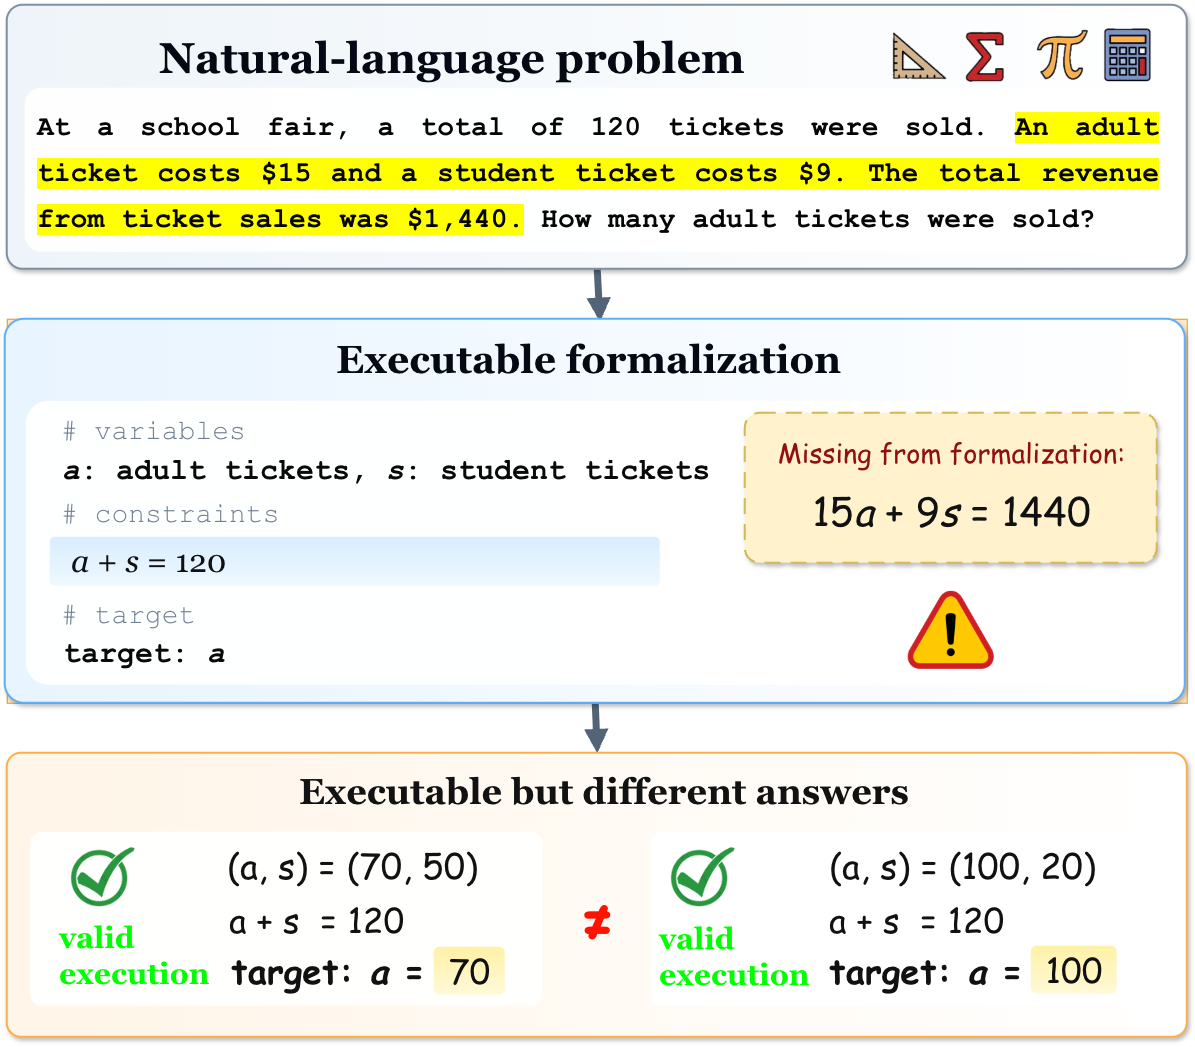
\includegraphics[width=\columnwidth]{figure/fig1.png}
\caption{An executable but target-ambiguous formalization caused by an omitted constraint.}
\Description{A natural-language ticket-sales problem is translated into an incomplete executable formalization containing only a plus s equals 120 and target a. The omitted revenue constraint is 15a plus 9s equals 1440. Although the program executes successfully, two feasible assignments, a equals 60 and a equals 100, produce different target values, showing that executability does not imply target determinacy.}
\label{fig:motivation}
\end{figure}

Figure~\ref{fig:motivation} illustrates the failure mode.  The source states both the total number of tickets and the total revenue, but the executable formalization retains only $a+s=120$.  Both $(a,s)=(60,60)$ and $(100,20)$ satisfy this incomplete model while giving different values of the requested number of adult tickets.  We call this condition \emph{target ambiguity}: feasible assignments disagree on the requested quantity.  It concerns the target rather than uniqueness of the entire assignment, since freedom in other variables need not affect the answer.

Detecting ambiguity does not establish how to resolve it.  The same model faithfully represents the shorter source ``Ten tasks are divided between A and B. How many does A receive?''  For the complete source, adding $a=b+2$ recovers an omitted relation; for the shorter source, the same addition fabricates information.  The formalization and solver verdict are identical, but the correct action changes with source support.  A repair policy must therefore distinguish evidence that the target is ambiguous from evidence that a particular constraint is justified.

We propose \method{}, a neuro-symbolic framework that separates these two decisions.  It first constructs two renamed copies of a generated specification and asks whether both can satisfy the constraints while disagreeing on the target.  A satisfying query provides auditable evidence of ambiguity.  The agent then proposes a constraint with supporting source text, and acceptance checks require consistency, non-redundancy, and restored target determinacy.  If no admissible repair is found, the agent abstains.  The solver guarantee concerns the encoded specification: even a determinate target can be wrong when the target or constraints were mistranslated.

We evaluate this framework at two complementary levels.  A controlled paired benchmark holds the formalization and diagnostic fixed while varying source support, testing whether the policy repairs a supported omission and abstains on its underspecified counterpart.  Human-verified natural-error studies then examine representation coverage, ambiguity detection, and successful grounded repair separately.  The controlled results show improved repair-or-abstain decisions, while the natural errors expose a substantial gap between detecting ambiguity and repairing its cause.  We also test whether concrete witness assignments improve decisions beyond the solver verdict.  In all experiments, DeGro is evaluated conditional on the source problem and an available candidate \textsc{ModelSpec}; we do not evaluate executable-code generation or a code-to-\textsc{ModelSpec} adapter, and therefore make no end-to-end improvement claim over SymCode.

\par\addvspace{9pt}
\begingroup
\setlength{\parskip}{5pt}
\noindent\textbf{Our research questions are:}

\noindent\textbf{(RQ1) Decision quality and tradeoffs.} How do target-determinacy diagnosis and source grounding affect repair-or-abstain accuracy and the tradeoff between supported repair and unsupported additions?

\noindent\textbf{(RQ2) Paired source sensitivity.} When the formalization and diagnostic are held fixed, can an agent both repair the source-supported omission and abstain on the underspecified member of the same pair?

\noindent\textbf{(RQ3) Practical bottlenecks.} How do representation coverage, ambiguity detection, and grounded repair limit effectiveness on natural errors, and do concrete witnesses improve controlled repair decisions beyond the verdict?
\par
\endgroup
\par\addvspace{10pt}

\takeaway{DeGro checks whether the encoded constraints determine the requested target, requires cited support and formal validation for repairs, and otherwise abstains.}

\par\addvspace{5pt}
\begingroup
\setlength{\parskip}{5pt}
\noindent\textbf{Our main contributions are:}

\noindent\textbf{(1) A target-determinacy-guided repair-or-abstain framework.} We introduce DeGro, which combines two-copy target-determinacy diagnosis with source-grounded repair, deterministic acceptance gates, and explicit abstention (RQ1).

\noindent\textbf{(2) Controlled and natural-source paired benchmarks.} We construct matched cases that hold the formalization fixed while varying whether the source supports the missing constraint. Alongside MIRA-Math, DRAW-Paired contributes 300 author-reviewed test pairs established from the beginning from natural algebra word problems, isolating supported repair from unsupported completion (RQ2).

\noindent\textbf{(3) A multi-stage empirical audit of executable reasoning.} We combine controlled and human-verified natural-error evaluations to separate representation coverage, ambiguity detection, and grounded repair; we additionally test whether concrete witnesses improve decisions (RQ3).

\noindent The formal guarantee concerns $F$; the empirical answers concern model and policy behavior.
\par
\endgroup

% Declare the pipeline boundary early to place it on page 3.
\begin{figure*}[!t]
\centering
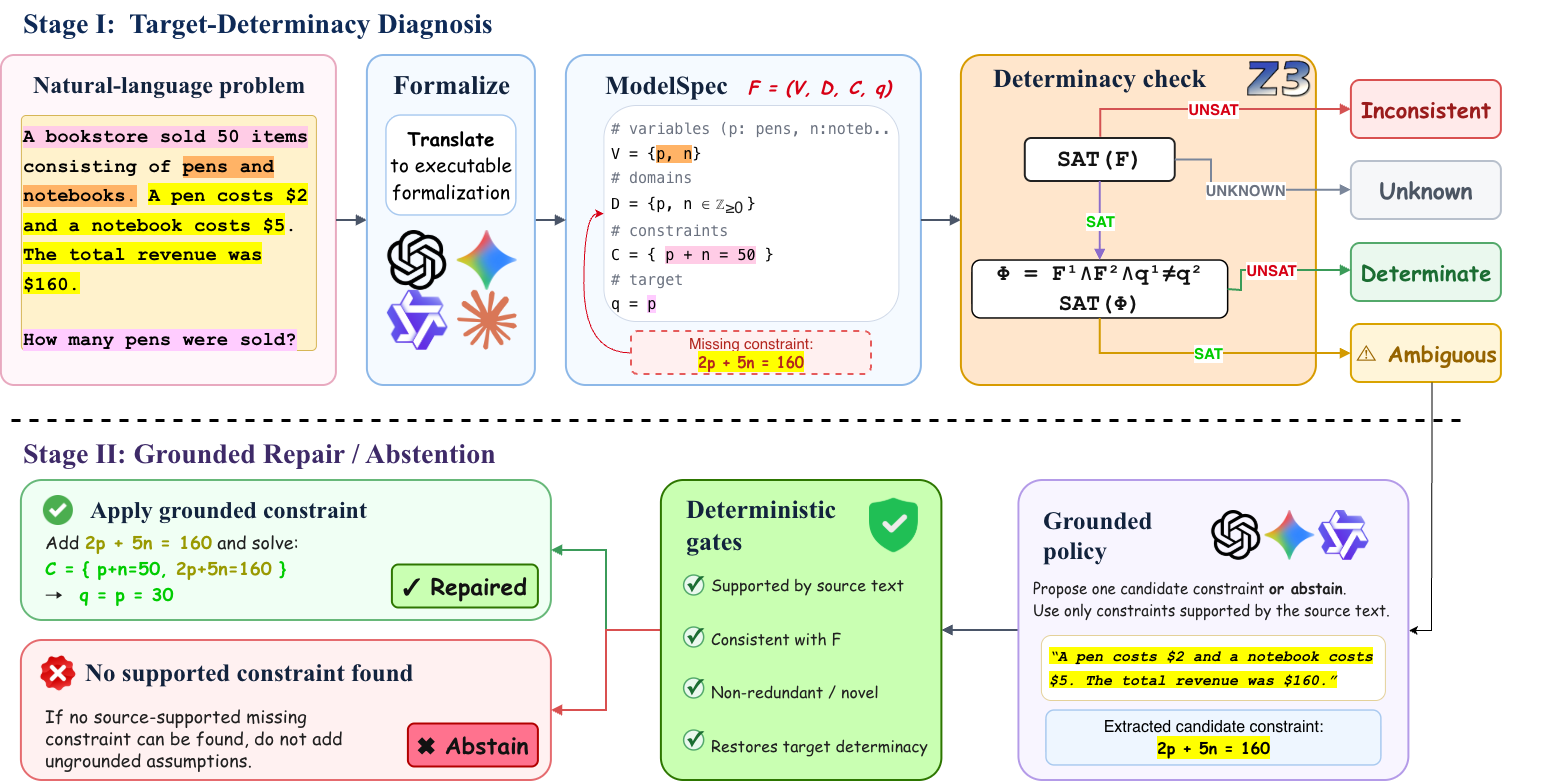
\includegraphics[width=\textwidth]{figure/pipeline-degro.png}
\caption{Overview of DeGro's target-determinacy diagnosis and grounded-repair pipeline.}
\Description{A two-stage pipeline diagram. A natural-language problem is translated by an upstream formalizer into a ModelSpec. Stage I checks satisfiability and compares the target across two renamed copies, producing inconsistent, unknown, determinate, or ambiguous. Ambiguous specifications enter Stage II, where a grounded policy extracts a source-supported candidate constraint. Deterministic gates check source support, consistency, novelty, and restored target determinacy, leading either to application of the constraint or to abstention.}
\label{fig:workflow}
\end{figure*}

\section{Related Work}
\subsection{Executable Mathematical Reasoning}
PAL and Program-of-Thoughts separate language-based reasoning from program execution to reduce computational errors~\cite{gao2023pal,chen2023pot}.  MathCoder and ToRA integrate code and tool calls into mathematical problem solving~\cite{wang2024mathcoder,gou2024tora}, while faithful chain-of-thought connects generated rationales to executable symbolic procedures~\cite{lyu2023faithful}.  SymCode is particularly close to our setting: it represents mathematical reasoning as a SymPy program and uses execution feedback to repair programmatic failures~\cite{nezhad2026symcode}.  These approaches motivate an additional check after successful execution.  A generated artifact may return a value even though its constraints admit other values of the requested quantity.  DeGro checks this property of the encoded feasible region and routes ambiguous specifications to grounded repair or abstention.  Integration with such systems requires an adapter that exposes their encoded variables, constraints, and target as a \textsc{ModelSpec}; evaluating that adapter and the resulting full pipeline is outside the present study.

Outcome verification and process supervision assess candidate solutions or intermediate reasoning steps~\cite{cobbe2021verifiers,uesato2022feedback,lightman2023verify}.  Self-Refine uses model-generated feedback, and CRITIC incorporates external tools into revision~\cite{madaan2023selfrefine,gou2024critic}; evidence on intrinsic self-correction shows the limits of revision without reliable external feedback~\cite{huang2024selfcorrect}.  DeGro contributes a specific solver observation: two feasible assignments disagree on the target.  This observation establishes ambiguity under the representation, independently of the predicted answer, but does not identify which source constraint should be added.

\subsection{Symbolic Diagnosis and Relational Verification}
Recent work addresses semantic failures that survive execution.  ReLoop tests optimization formulations through solver-based parameter perturbations~\cite{lian2026reloop}.  SymDiag translates reasoning steps into constraints and uses satisfiability and entailment checks to localize defects, with a Self-Auditor to distinguish translation errors from reasoning errors~\cite{cui2026symdiag}.  Minimal-core-guided repair instead returns an unsatisfiable subset of generated constraints as evidence for revising inconsistent translations~\cite{sarkar2026cores,liffiton2008mus}.  DeGro focuses on a complementary condition: the specification is satisfiable, but its feasible assignments disagree on the requested target.  Its diagnosis concerns the specification as a whole rather than the validity of individual derivation steps, and its additive repair policy requires support from the original source.

The two-copy construction builds on self-composition and product programs, which reduce relational verification to queries over renamed copies~\cite{barthe2004selfcomposition,terauchi2005safety,barthe2011product}.  DeGro instantiates this established technique as target agreement across feasible assignments.  Agreement on the target is weaker than uniqueness of the full assignment: nuisance variables may remain free without making the answer ambiguous.  Counterexample-guided refinement and synthesis likewise use solver evidence to guide changes~\cite{clarke2000cegar,solarlezama2006cegis}.  Here, however, a counterexample refutes target determinacy without supplying a semantically justified edit.  Our contribution is the integration of this diagnosis with a source-sensitive repair policy and its evaluation, rather than a new relational verification primitive.

\subsection{Grounded Repair, Abstention, and Faithfulness}
Classical diagnosis, abductive inference, and formal model repair provide foundations for identifying defects and modifying specifications to satisfy a desired property~\cite{reiter1987diagnosis,dillig2013abduction,attie2008modelrepair}.  LLM-based repair extends this direction to declarative formal specifications~\cite{alhanahnah2024alloyrepair}.  Restoring determinacy alone is insufficient in our setting, since a guessed equality can force a unique target.  DeGro therefore requests a source-supported constraint and checks consistency, non-redundancy, and restored determinacy before acceptance.  These formal gates verify the effect of the edit; source support remains a separate semantic requirement.

Selective prediction studies when to withhold an answer under a risk--coverage tradeoff~\cite{elyaniv2010foundations,geifman2017selective}, and semantic uncertainty estimates uncertainty in language-model outputs~\cite{kuhn2023semantic}.  DeGro bases its repair-or-abstain decision on two distinct questions: whether the encoded target is determinate and whether the source supports a constraint that resolves ambiguity.  MIRA-Math is directly relevant because it evaluates requesting and integrating necessary missing information~\cite{albateh2026mira}.  We adapt its validated latent states into matched sources with identical formalizations but different support for repair, isolating the decision to recover an omitted relation or abstain from unsupported completion.

Autoformalization also separates formal validity from preservation of natural-language meaning~\cite{wu2022autoformalization,azerbayev2023proofnet}.  DeGro's guarantee is similarly representation-relative: a determinate specification can still contain a wrong target or an unsupported constraint.  Our paired and human-verified natural-error evaluations therefore distinguish determinacy diagnosis, grounded repair, and answer accuracy rather than treating a solver verdict as proof of source-to-formal faithfulness.

\section{Methodology}
DeGro checks whether a candidate mathematical specification determines the requested target.  Its evaluated interface is the pair $(P,F)$: the source problem $P$ and an available \textsc{ModelSpec} $F$.  The upstream mechanism that produced $F$ may be a direct autoformalizer, a program adapter, or another reasoning system; it is not part of the controlled intervention evaluated here.  Stage I diagnoses target ambiguity using a symbolic solver. Stage II attempts to resolve an ambiguous target by adding a constraint with source provenance, or abstains if no candidate is accepted. Figure~\ref{fig:workflow} summarizes this component boundary.

\subsection{Problem Setup and Target Determinacy}
Given a natural-language problem $P$ and a candidate specification $F=(V,D,C,q)$, $V$ is the set of variables, $D$ their domains, $C$ the constraints, and $q(V)$ the requested expression. Its feasible assignments are
\begin{equation}
\mathrm{Sol}(F)=\{m\mid m\models D\land C\}.
\label{eq:solutions}
\end{equation}
For a satisfiable $F$, the target is \emph{determinate} when every feasible assignment gives the same target value:
\begin{equation}
\mathrm{Det}(F,q)\iff
\forall m_1,m_2\in\mathrm{Sol}(F),\quad q(m_1)=q(m_2).
\label{eq:determinacy}
\end{equation}
Target determinacy does not require a unique assignment to all variables. For example, $x=5,y\geq0$ fixes the target $q=x$ even though $y$ remains free. An inconsistent specification is reported separately and never receives a determinacy certificate.

The specification is stored as a typed \textsc{ModelSpec}: a structured record of variable sorts and bounds, source-linked constraints, and the target. Computational and verification backends consume this same representation, avoiding discrepancies between independently generated programs. The supported fragment includes integer, real, and Boolean variables, arithmetic equalities and inequalities, finite domains, and selected modular constraints.

The certificate concerns $F$, not whether $F$ correctly represents $P$. Wrong or extra constraints can fix a target while mistranslating the source. DeGro therefore repairs only ambiguous specifications by adding constraints; correcting a determinate but incorrect representation is outside its scope.

\subsection{Stage I: Target-Determinacy Diagnosis}
DeGro first checks whether $D\land C$ is satisfiable. An unsatisfiable result yields \textsc{inconsistent}; a timeout or inconclusive solver result yields \textsc{unknown}. If the specification is satisfiable, DeGro constructs two copies with disjoint variable names and asks whether they can produce different target values:
\begin{equation}
\Phi(F,q)=F^{(1)}\land F^{(2)}\land
q(V^{(1)})\neq q(V^{(2)}).
\label{eq:query}
\end{equation}
If $\Phi$ is satisfiable, its projections form a \emph{target-divergent witness pair}, and the status is \textsc{ambiguous}. If $\Phi$ is unsatisfiable, the status is \textsc{determinate}, since the initial check has already established that $F$ has a solution. Unsupported representations yield \textsc{unsupported} before solver verification. Only \textsc{ambiguous} enters Stage II.

\begin{algorithm}[H]
\caption{Target-determinacy verification}
\label{alg:verify}
\footnotesize
\begin{algorithmic}[1]
\Require Typed specification $F=(V,D,C,q)$
\Ensure Status and optional witness pair
\State $r_0 \gets \Call{CheckSat}{D\land C}$
\State \textbf{if} $r_0=\textsc{unsat}$ \textbf{return} \textsc{inconsistent}
\State \textbf{if} $r_0\neq\textsc{sat}$ \textbf{return} \textsc{unknown}
\State $\Phi\gets F^{(1)}\land F^{(2)}\land(q^{(1)}\neq q^{(2)})$ using disjoint copies
\State $(r_1,M) \gets \Call{CheckSat}{\Phi}$
\State \textbf{if} $r_1=\textsc{unsat}$ \textbf{return} \textsc{determinate}
\State \textbf{if} $r_1\neq\textsc{sat}$ \textbf{return} \textsc{unknown}
\State \Return $\textsc{ambiguous},\Call{ProjectWitnesses}{M}$
\end{algorithmic}
\end{algorithm}

\paragraph{Soundness.}
Assuming semantics-preserving compilation and a sound solver for the supported theory, $\mathrm{SAT}(F)$ together with $\mathrm{UNSAT}(\Phi)$ establishes target determinacy: any two feasible assignments with different targets would satisfy Eq.~\eqref{eq:query}, contradicting unsatisfiability. Conversely, a satisfying assignment to $\Phi$ supplies two feasible witnesses with different targets. Timeout and \textsc{unknown} provide no certificate. The implementation uses a restricted expression compiler and separate variable maps for the two Z3 copies~\cite{demoura2008z3}.

\subsection{Stage II: Grounded Repair or Abstention}
The verifier retains the target-divergent witness pair as a certificate, but the default repair prompt receives only the source problem, the encoded constraints and target, and the typed \textsc{ambiguous} verdict. It returns either \textsc{add-constraint} with an exact supporting source span (or a permitted domain rule), or \textsc{abstain}. It receives neither the hidden gold target nor the missing gold constraint. An additional ablation exposes the concrete witnesses to test whether their values help beyond the verdict; they do not improve decisions on the present benchmark. In either variant, the model must recover a relation from the source rather than select a witness as correct.

\paragraph{Acceptance gate.}
For a proposed constraint $c$ and a frozen set $\mathcal{R}$ of permitted domain-semantics rules, the deterministic gate accepts $c$ only when
\begin{align}
\mathrm{Accept}(c)\iff{}&\mathrm{Compiles}(c)\land
\mathrm{Provenance}(c,P,\mathcal{R})\nonumber\\
&\land\mathrm{SAT}(F\land c)\land\neg(F\models c)
\land\mathrm{Det}(F\land c,q).
\label{eq:accept}
\end{align}
These checks require that the candidate compile, cite a source span occurring in $P$ or a rule in $\mathcal{R}$, preserve consistency, add a non-redundant restriction, and restore target determinacy. Compilation failures and inconclusive checks do not permit acceptance.

Provenance is an auditable check, not a proof that the constraint correctly expresses the cited text. Passing the gate therefore establishes valid provenance and determinacy under the repaired specification, rather than semantic correctness with respect to $P$. Semantic source support and functional correctness are evaluated separately for repair credit; an incorrect translation or unsupported target pin does not earn credit merely by passing the gate.

\paragraph{Bounded repair.}
DeGro allows at most two proposal attempts. The first accepted constraint is committed and terminates the loop. If the first proposal is rejected, the second attempt receives the rejection reason and operates on the unchanged $F$. Rejected constraints are not accumulated: each candidate must restore determinacy on its own, and a supported but insufficient addition is rejected. If the model abstains or neither candidate passes, the outcome is \textsc{no-admissible-repair-found}, and $F$ is preserved.

Failure to find an admissible repair does not prove that the source is underspecified: the model may have missed a relation already present in the source.

\paragraph{Controller policy.}
Table~\ref{tab:policy} maps verifier states to agent actions. A determinate result permits an answer scoped to the current specification, including an accepted repair when present. In interactive use, failure to find a repair can trigger clarification or abstention; the benchmark scores abstention because no clarification channel is available. Inconsistent, unknown, and unsupported states require distinct fallbacks rather than being treated as ambiguous inputs. The parser, compiler, solver, and gate form the trusted boundary; the language model only proposes specifications and repairs. Logs retain solver verdicts, witnesses, proposals, cited support, and rejection reasons for auditing.

\begin{table}[t]
\centering
\caption{Controller semantics for DeGro integration.}
\label{tab:policy}
\small
\begin{tabular}{lll}
\toprule
Verifier state & Evidence & Controller action\\
\midrule
Determinate & $F$ sat, $\Phi$ unsat & answer with scope\\
Ambiguous & targets disagree & grounded repair\\
Inconsistent & $F$ unsat & revise encoding\\
Unknown & solver inconclusive & fallback/escalate\\
Unsupported & outside fragment & alternate tool\\
No repair found & no accepted candidate & ask or abstain\\
\bottomrule
\end{tabular}
\end{table}



\section{Experiments and Results}
\subsection{Setup}
\subsubsection{Evaluation Scope}
We evaluate repair policies along three complementary dimensions: (i) \emph{diagnostic guidance}, whether a solver-produced target-ambiguity verdict improves revision; (ii) \emph{source grounding}, whether exact source evidence prevents unsupported additions; and (iii) \emph{repair-or-abstain behavior}, whether a policy repairs a supported omission while withholding an edit when the source is genuinely underspecified. The first two dimensions address RQ1, whereas repair-or-abstain behavior on matched sources directly addresses RQ2.

\subsubsection{Baselines}
To evaluate the effectiveness of \method{}, we compare it against representative repair policies that use weaker diagnostic or grounding signals. All methods receive the same source, current constraints, and target; begin from the same initial formalization; and use a two-attempt repair budget. Differences therefore reflect the feedback and repair policy rather than initial-generation quality. We consider the following baselines:
\begin{itemize}
    \item \textbf{Self-review.} The model revises the formalization using the source and current artifact, but receives no explicit solver diagnosis and is not required to ground an added constraint in the source.
    \item \textbf{Grounded self-review.} The model follows the same exact-span grounding rule used by \method{}, so every introduced constraint must cite supporting source text. It receives no solver feedback, isolating grounding without determinacy guidance.
    \item \textbf{Determinacy-guided repair.} The model receives the typed \textsc{ambiguous} verdict but no exact-span grounding requirement. This baseline isolates the effect of determinacy feedback without source-grounded control.
\end{itemize}

\subsubsection{Models}
We evaluate all four policies with GPT-OSS 20B and GPT-OSS 120B~\cite{openai2025gptoss}, and Nemotron 3 Nano 30B~\cite{nvidia2025nemotronnano}. All models use the same cases, frozen prompt, temperature 1.0, and repair budget.

\subsubsection{Metrics}
\noindent\textbf{Accuracy.} Our primary metric counts a decision as correct when the method produces a grounded, functionally correct repair for an omission case or abstains on an underspecified case. Because each controlled pair contains one case of each type, accuracy is equivalently computed as
\[
\mathrm{Accuracy}=\frac{\mathrm{Recall}+\mathrm{Specificity}}{2}.
\]
\noindent\textbf{Recall and specificity.} Recall measures the proportion of omission cases repaired correctly, whereas specificity measures the proportion of underspecified cases on which the method correctly abstains. We omit the false-positive rate because it is exactly $1-\mathrm{Specificity}$.

\noindent\textbf{Unsupported repair rate.} URR is the share of proposed additions lacking source support and is reported with recall to account for abstention. Semantic, functional, and grounded outcomes remain separate. Accuracy comparisons use exact paired McNemar tests with Holm correction across models; percentage-point intervals use 10,000 pair-cluster bootstrap resamples.

\subsection{Datasets}
We evaluate on two matched-pair benchmarks: 360 MIRA-Math pairs across six controlled mathematical families and 300 DRAW-Paired test pairs derived from natural algebra word problems. Figure~\ref{fig:dataset_composition} summarizes their composition.

\begin{figure}[t]
\centering
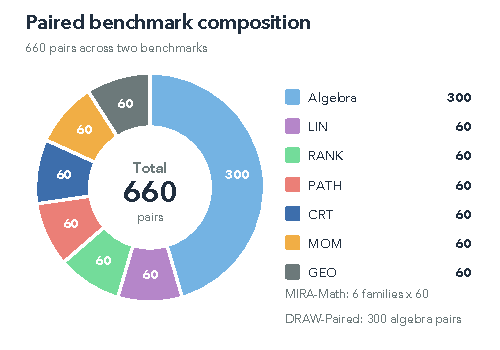
\includegraphics[width=\columnwidth]{figure/dataset_composition.pdf}
\caption{Paired benchmark composition. DRAW-Paired contributes 300 pairs constructed from natural algebra word-problem sources; MIRA-Math contributes six 60-pair families: linear separation (LIN), rank-deficient systems (RANK), path sums (PATH), Chinese-remainder reconstruction (CRT), moment constraints (MOM), and geometry (GEO). Every pair yields one \textsc{omission} and one \textsc{underspecified} case.}
\Description{A donut chart shows 660 pairs: 300 algebra word-problem pairs from DRAW-Paired and 60 pairs from each of the six MIRA-Math families.}
\label{fig:dataset_composition}
\end{figure}

Both benchmarks use the same construction. Removing one target-critical constraint yields a satisfiable but target-ambiguous specification shared by both members of a pair. The \textsc{omission} source retains the supporting fact and should be repaired; the \textsc{underspecified} source removes it and should trigger abstention. In MIRA-Math, the missing fact is provided by the dataset and every retained pair passes satisfiability, ambiguity, and restored-determinacy checks~\cite{albateh2026mira}. DRAW-Paired applies this design to 300 author-reviewed test pairs constructed from natural algebra word problems in DRAW-1K~\cite{upadhyay2017derivations} from the beginning. All supporting spans and deletions were author-reviewed. Full split, filtering, and provenance details are reported in the supplement.

\subsection{Main Paired Results}

\begin{table*}[t]
\centering
\caption{Main paired experiments on MIRA-360 (360 pairs, 720 cases across six families) and DRAW-Paired (300 author-reviewed test pairs, 600 cases). Values are percentages. Accuracy is primary; recall and specificity decompose repair and abstention, and URR measures unsupported additions among proposed additions. Blue rows denote DeGro; bold accuracy marks the best policy within each model and dataset.}
\label{tab:main}
\label{tab:draw_paired}
\fontsize{8.5}{10}\selectfont
\setlength{\tabcolsep}{4pt}
\renewcommand{\arraystretch}{1.12}
\begin{tabularx}{.98\textwidth}{ll|*{4}{>{\centering\arraybackslash}X}|*{4}{>{\centering\arraybackslash}X}}
\toprule
 & & \multicolumn{4}{c}{\textbf{MIRA-Math}} & \multicolumn{4}{c}{\textbf{DRAW-Paired}}\\
\cmidrule(lr){3-6}\cmidrule(lr){7-10}
\textbf{Model} & \textbf{Method} & Acc.$\uparrow$ & Recall$\uparrow$ & Spec.$\uparrow$ & URR$\downarrow$ & Acc.$\uparrow$ & Recall$\uparrow$ & Spec.$\uparrow$ & URR$\downarrow$\\
\midrule
GPT-OSS & Self-review & 90.6 & 93.1 & 88.1 & 14.5 & 73.8 & 66.7 & 81.0 & 43.3\\
20B & Grounded self-review & 91.7 & 94.7 & 88.6 & 11.2 & 73.3 & 62.3 & 84.3 & 43.8\\
 & Determinacy-guided & 92.6 & 88.1 & 97.2 & 7.9 & 73.7 & 57.0 & 90.3 & 46.1\\
 & \cellcolor{degrotableblue}\textbf{DeGro (ours)} & \cellcolor{degrotableblue}\textbf{96.3} & \cellcolor{degrotableblue}93.3 & \cellcolor{degrotableblue}99.2 & \cellcolor{degrotableblue}2.9 & \cellcolor{degrotableblue}\textbf{79.2} & \cellcolor{degrotableblue}66.7 & \cellcolor{degrotableblue}91.7 & \cellcolor{degrotableblue}36.3\\
\midrule
GPT-OSS & Self-review & 78.6 & 99.4 & 57.8 & 29.9 & 72.0 & 68.3 & 75.7 & 44.1\\
120B & Grounded self-review & 89.6 & 96.7 & 82.5 & 15.5 & 69.0 & 54.0 & 84.0 & 51.1\\
 & Determinacy-guided & 92.4 & 98.6 & 86.1 & 13.4 & \textbf{77.8} & 69.3 & 86.3 & 37.5\\
 & \cellcolor{degrotableblue}\textbf{DeGro (ours)} & \cellcolor{degrotableblue}\textbf{96.1} & \cellcolor{degrotableblue}97.8 & \cellcolor{degrotableblue}94.4 & \cellcolor{degrotableblue}6.4 & \cellcolor{degrotableblue}\textbf{77.8} & \cellcolor{degrotableblue}63.7 & \cellcolor{degrotableblue}92.0 & \cellcolor{degrotableblue}38.8\\
\midrule
Nemotron & Self-review & 83.9 & 76.1 & 91.7 & 25.5 & 63.5 & 44.7 & 82.3 & 59.0\\
Nano 30B & Grounded self-review & 86.7 & 75.0 & 98.3 & 4.6 & 60.7 & 35.7 & 85.7 & 61.9\\
 & Determinacy-guided & 72.9 & 53.9 & 91.9 & 27.3 & 63.3 & 34.7 & 92.0 & 55.4\\
 & \cellcolor{degrotableblue}\textbf{DeGro (ours)} & \cellcolor{degrotableblue}\textbf{89.6} & \cellcolor{degrotableblue}79.4 & \cellcolor{degrotableblue}99.7 & \cellcolor{degrotableblue}1.0 & \cellcolor{degrotableblue}\textbf{70.8} & \cellcolor{degrotableblue}48.3 & \cellcolor{degrotableblue}93.3 & \cellcolor{degrotableblue}44.4\\
\bottomrule
\end{tabularx}
\end{table*}

\paragraph{MIRA-Math.}
Table~\ref{tab:main} reports the MIRA-Math aggregate. DeGro achieves the highest accuracy for all three models, improving over grounded self-review by 2.9--6.5 points; all comparisons remain significant after Holm correction. Full confidence intervals and tests appear in the supplement.


\begin{comment}
\begin{figure*}[t]
\centering
\begin{minipage}[t]{.32\textwidth}\centering
\textbf{(a) Final decision accuracy}\par\smallskip
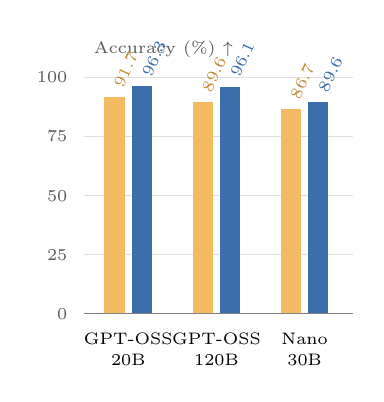
\begin{tikzpicture}[x=1.12cm,y=.03cm,font=\scriptsize]
\draw[black!12] (0,0) -- (3.05,0); \node[anchor=east,font=\fontsize{6.5}{7.5}\selectfont,text=black!65] at (-.08,0) {0};
\draw[black!12] (0,25) -- (3.05,25); \node[anchor=east,font=\fontsize{6.5}{7.5}\selectfont,text=black!65] at (-.08,25) {25};
\draw[black!12] (0,50) -- (3.05,50); \node[anchor=east,font=\fontsize{6.5}{7.5}\selectfont,text=black!65] at (-.08,50) {50};
\draw[black!12] (0,75) -- (3.05,75); \node[anchor=east,font=\fontsize{6.5}{7.5}\selectfont,text=black!65] at (-.08,75) {75};
\draw[black!12] (0,100) -- (3.05,100); \node[anchor=east,font=\fontsize{6.5}{7.5}\selectfont,text=black!65] at (-.08,100) {100};
\node[anchor=west,font=\fontsize{6.5}{7.5}\selectfont,text=black!65] at (0,112) {Accuracy (\%) $\uparrow$};
\fill[degroorange!85] (0.22999999999999998,0) rectangle (0.46,91.7);
\fill[degroblue] (0.54,0) rectangle (0.77,96.3);
\node[above,font=\fontsize{6.5}{7.5}\selectfont,text=degroorange!80!black,rotate=65,anchor=west] at (0.33999999999999997,92.7) {91.7};
\node[above,font=\fontsize{6.5}{7.5}\selectfont,text=degroblue,rotate=65,anchor=west] at (0.66,97.3) {96.3};
\node[align=center,font=\fontsize{6.5}{7.5}\selectfont,anchor=north] at (0.5,-4) {GPT-OSS\\20B};
\fill[degroorange!85] (1.23,0) rectangle (1.46,89.6);
\fill[degroblue] (1.54,0) rectangle (1.77,96.1);
\node[above,font=\fontsize{6.5}{7.5}\selectfont,text=degroorange!80!black,rotate=65,anchor=west] at (1.34,90.6) {89.6};
\node[above,font=\fontsize{6.5}{7.5}\selectfont,text=degroblue,rotate=65,anchor=west] at (1.66,97.1) {96.1};
\node[align=center,font=\fontsize{6.5}{7.5}\selectfont,anchor=north] at (1.5,-4) {GPT-OSS\\120B};
\fill[degroorange!85] (2.23,0) rectangle (2.46,86.7);
\fill[degroblue] (2.54,0) rectangle (2.77,89.6);
\node[above,font=\fontsize{6.5}{7.5}\selectfont,text=degroorange!80!black,rotate=65,anchor=west] at (2.34,87.7) {86.7};
\node[above,font=\fontsize{6.5}{7.5}\selectfont,text=degroblue,rotate=65,anchor=west] at (2.66,90.6) {89.6};
\node[align=center,font=\fontsize{6.5}{7.5}\selectfont,anchor=north] at (2.5,-4) {Nano\\30B};
\draw[black!50] (0,0) -- (3.05,0);
\end{tikzpicture}\end{minipage}\hfill
\begin{minipage}[t]{.32\textwidth}\centering
\textbf{(b) Grounded repair success}\par\smallskip
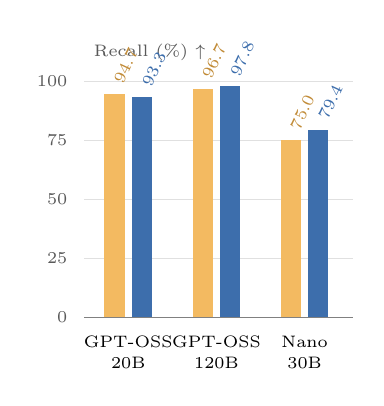
\begin{tikzpicture}[x=1.12cm,y=.03cm,font=\scriptsize]
\draw[black!12] (0,0) -- (3.05,0); \node[anchor=east,font=\fontsize{6.5}{7.5}\selectfont,text=black!65] at (-.08,0) {0};
\draw[black!12] (0,25) -- (3.05,25); \node[anchor=east,font=\fontsize{6.5}{7.5}\selectfont,text=black!65] at (-.08,25) {25};
\draw[black!12] (0,50) -- (3.05,50); \node[anchor=east,font=\fontsize{6.5}{7.5}\selectfont,text=black!65] at (-.08,50) {50};
\draw[black!12] (0,75) -- (3.05,75); \node[anchor=east,font=\fontsize{6.5}{7.5}\selectfont,text=black!65] at (-.08,75) {75};
\draw[black!12] (0,100) -- (3.05,100); \node[anchor=east,font=\fontsize{6.5}{7.5}\selectfont,text=black!65] at (-.08,100) {100};
\node[anchor=west,font=\fontsize{6.5}{7.5}\selectfont,text=black!65] at (0,112) {Recall (\%) $\uparrow$};
\fill[degroorange!85] (0.22999999999999998,0) rectangle (0.46,94.7);
\fill[degroblue] (0.54,0) rectangle (0.77,93.3);
\node[above,font=\fontsize{6.5}{7.5}\selectfont,text=degroorange!80!black,rotate=65,anchor=west] at (0.33999999999999997,95.7) {94.7};
\node[above,font=\fontsize{6.5}{7.5}\selectfont,text=degroblue,rotate=65,anchor=west] at (0.66,94.3) {93.3};
\node[align=center,font=\fontsize{6.5}{7.5}\selectfont,anchor=north] at (0.5,-4) {GPT-OSS\\20B};
\fill[degroorange!85] (1.23,0) rectangle (1.46,96.7);
\fill[degroblue] (1.54,0) rectangle (1.77,97.8);
\node[above,font=\fontsize{6.5}{7.5}\selectfont,text=degroorange!80!black,rotate=65,anchor=west] at (1.34,97.7) {96.7};
\node[above,font=\fontsize{6.5}{7.5}\selectfont,text=degroblue,rotate=65,anchor=west] at (1.66,98.8) {97.8};
\node[align=center,font=\fontsize{6.5}{7.5}\selectfont,anchor=north] at (1.5,-4) {GPT-OSS\\120B};
\fill[degroorange!85] (2.23,0) rectangle (2.46,75.0);
\fill[degroblue] (2.54,0) rectangle (2.77,79.4);
\node[above,font=\fontsize{6.5}{7.5}\selectfont,text=degroorange!80!black,rotate=65,anchor=west] at (2.34,76.0) {75.0};
\node[above,font=\fontsize{6.5}{7.5}\selectfont,text=degroblue,rotate=65,anchor=west] at (2.66,80.4) {79.4};
\node[align=center,font=\fontsize{6.5}{7.5}\selectfont,anchor=north] at (2.5,-4) {Nano\\30B};
\draw[black!50] (0,0) -- (3.05,0);
\end{tikzpicture}\end{minipage}\hfill
\begin{minipage}[t]{.32\textwidth}\centering
\textbf{(c) Correct abstention}\par\smallskip
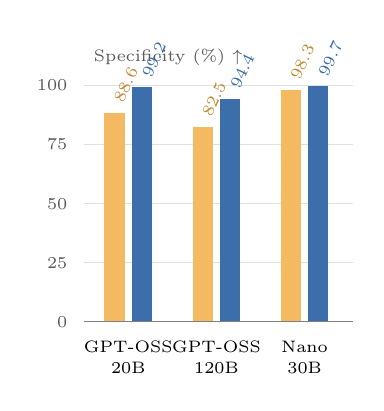
\begin{tikzpicture}[x=1.12cm,y=.03cm,font=\scriptsize]
\draw[black!12] (0,0) -- (3.05,0); \node[anchor=east,font=\fontsize{6.5}{7.5}\selectfont,text=black!65] at (-.08,0) {0};
\draw[black!12] (0,25) -- (3.05,25); \node[anchor=east,font=\fontsize{6.5}{7.5}\selectfont,text=black!65] at (-.08,25) {25};
\draw[black!12] (0,50) -- (3.05,50); \node[anchor=east,font=\fontsize{6.5}{7.5}\selectfont,text=black!65] at (-.08,50) {50};
\draw[black!12] (0,75) -- (3.05,75); \node[anchor=east,font=\fontsize{6.5}{7.5}\selectfont,text=black!65] at (-.08,75) {75};
\draw[black!12] (0,100) -- (3.05,100); \node[anchor=east,font=\fontsize{6.5}{7.5}\selectfont,text=black!65] at (-.08,100) {100};
\node[anchor=west,font=\fontsize{6.5}{7.5}\selectfont,text=black!65] at (0,112) {Specificity (\%) $\uparrow$};
\fill[degroorange!85] (0.22999999999999998,0) rectangle (0.46,88.6);
\fill[degroblue] (0.54,0) rectangle (0.77,99.2);
\node[above,font=\fontsize{6.5}{7.5}\selectfont,text=degroorange!80!black,rotate=65,anchor=west] at (0.33999999999999997,89.6) {88.6};
\node[above,font=\fontsize{6.5}{7.5}\selectfont,text=degroblue,rotate=65,anchor=west] at (0.66,100.2) {99.2};
\node[align=center,font=\fontsize{6.5}{7.5}\selectfont,anchor=north] at (0.5,-4) {GPT-OSS\\20B};
\fill[degroorange!85] (1.23,0) rectangle (1.46,82.5);
\fill[degroblue] (1.54,0) rectangle (1.77,94.4);
\node[above,font=\fontsize{6.5}{7.5}\selectfont,text=degroorange!80!black,rotate=65,anchor=west] at (1.34,83.5) {82.5};
\node[above,font=\fontsize{6.5}{7.5}\selectfont,text=degroblue,rotate=65,anchor=west] at (1.66,95.4) {94.4};
\node[align=center,font=\fontsize{6.5}{7.5}\selectfont,anchor=north] at (1.5,-4) {GPT-OSS\\120B};
\fill[degroorange!85] (2.23,0) rectangle (2.46,98.3);
\fill[degroblue] (2.54,0) rectangle (2.77,99.7);
\node[above,font=\fontsize{6.5}{7.5}\selectfont,text=degroorange!80!black,rotate=65,anchor=west] at (2.34,99.3) {98.3};
\node[above,font=\fontsize{6.5}{7.5}\selectfont,text=degroblue,rotate=65,anchor=west] at (2.66,100.7) {99.7};
\node[align=center,font=\fontsize{6.5}{7.5}\selectfont,anchor=north] at (2.5,-4) {Nano\\30B};
\draw[black!50] (0,0) -- (3.05,0);
\end{tikzpicture}\end{minipage}
\par\smallskip
{\small\textcolor{degroorange!85}{\rule{9pt}{5pt}}\ Grounded self-review\qquad\textcolor{degroblue}{\rule{9pt}{5pt}}\ DeGro}
\caption{MIRA-360 results. DeGro has higher accuracy than grounded self-review for all three models after Holm correction. Recall and specificity expose model-specific tradeoffs. All axes start at zero.}
\Description{Three grouped bar charts compare grounded self-review in orange and DeGro in blue for GPT-OSS 20B, GPT-OSS 120B, and Nemotron Nano 30B. Panels show accuracy, recall, and specificity, with numerical labels and zero-based percentage axes.}
\label{fig:result_summary}
\end{figure*}
\end{comment}


\paragraph{Grounding trade-off.}
DeGro lowers URR and raises specificity for all three models while broadly preserving recall. Thus the reduction in unsupported additions does not merely reflect universal abstention.

\begin{comment}
\begin{figure*}[t]
\centering
\begin{tcolorbox}[
  enhanced,width=.98\textwidth,
  colback=degrolight,colframe=degrogray!75,
  boxrule=.7pt,arc=3pt,
  left=8pt,right=8pt,top=6pt,bottom=6pt,
  title={\bfseries\small Case \texttt{lin-000271}: same query, same formalization},
  colbacktitle=degrogray!12,coltitle=black,
  toptitle=3pt,bottomtitle=3pt
]
\begin{minipage}[t]{.75\linewidth}\vspace{0pt}
{\scriptsize\bfseries\textcolor{degrogray}{SOURCE PROBLEM}}\par
\smallskip
{\small $-2a+3b-4c=15,\qquad -a+2b+4c=-8.$\quad Find the integer value of $a$.}\par
\medskip
{\scriptsize\bfseries\textcolor{degrogray}{CURRENT ENCODING}}\par
{\small The two displayed equations; $a,b,c\in\mathbb{Z}$ is already enforced.}
\end{minipage}\hfill
\begin{minipage}[t]{.21\linewidth}\vspace{0pt}
\begin{tcolorbox}[
  colback=degroorange!10,colframe=degroorange!85!black,
  boxrule=.8pt,arc=3pt,left=4pt,right=4pt,top=5pt,bottom=5pt
]
\centering
{\scriptsize\bfseries SOLVER VERDICT}\par\smallskip
{\small\bfseries\textcolor{degroorange!85!black}{AMBIGUOUS}}\par
{\tiny Multiple feasible values of $a$}
\end{tcolorbox}
\end{minipage}
\end{tcolorbox}

\vspace{2pt}
{\scriptsize\textcolor{degrogray}{Each policy receives the identical source, encoded constraints, and ambiguity verdict.}}\par
\vspace{4pt}

\begin{minipage}[t]{.238\textwidth}
\begin{tcolorbox}[
  enhanced,height=34mm,valign=top,
  colback=white,colframe=degrogray!65,boxrule=.65pt,arc=3pt,
  left=6pt,right=6pt,top=5pt,bottom=5pt,
  title={\small\bfseries Self-Review},
  colbacktitle=degrogray!10,coltitle=black,
  toptitle=3pt,bottomtitle=3pt
]
{\fontsize{6.8}{8}\selectfont\bfseries\textcolor{degrogray}{PROPOSED EDIT}}\par
{\scriptsize\ttfamily ADD\_CONSTRAINT}\par
\smallskip
\centering{\small $a=\operatorname{int}(a)$}\par
\smallskip
\raggedright{\fontsize{7.2}{8.4}\selectfont Repeats the declared integer domain; ambiguity remains.}\par
\vfill
\textcolor{red!75!black}{\bfseries\scriptsize $\times$ REJECTED}
\end{tcolorbox}
\end{minipage}\hfill
\begin{minipage}[t]{.238\textwidth}
\begin{tcolorbox}[
  enhanced,height=34mm,valign=top,
  colback=white,colframe=degroorange!80!black,boxrule=.65pt,arc=3pt,
  left=6pt,right=6pt,top=5pt,bottom=5pt,
  title={\small\bfseries Grounded Self-Review},
  colbacktitle=degroorange!10,coltitle=black,
  toptitle=3pt,bottomtitle=3pt
]
{\fontsize{6.8}{8}\selectfont\bfseries\textcolor{degrogray}{PROPOSED EDIT}}\par
{\scriptsize\ttfamily ADD\_CONSTRAINT}\par
\smallskip
\centering{\small $a=\operatorname{int}(a)$}\par
\smallskip
\raggedright{\fontsize{7.2}{8.4}\selectfont Cites \emph{integer value}, but adds no missing relation.}\par
\vfill
\textcolor{red!75!black}{\bfseries\scriptsize $\times$ REJECTED}
\end{tcolorbox}
\end{minipage}\hfill
\begin{minipage}[t]{.238\textwidth}
\begin{tcolorbox}[
  enhanced,height=34mm,valign=top,
  colback=white,colframe=degroorange!80!black,boxrule=.65pt,arc=3pt,
  left=6pt,right=6pt,top=5pt,bottom=5pt,
  title={\small\bfseries Determinacy-Guided},
  colbacktitle=degroorange!10,coltitle=black,
  toptitle=3pt,bottomtitle=3pt
]
{\fontsize{6.8}{8}\selectfont\bfseries\textcolor{degrogray}{PROPOSED EDIT}}\par
{\scriptsize\ttfamily ADD\_CONSTRAINT}\par
\smallskip
\centering{\small $a\bmod 1=0$}\par
\smallskip
\raggedright{\fontsize{7.2}{8.4}\selectfont Reacts to ambiguity, but invents no source-supported relation.}\par
\vfill
\textcolor{red!75!black}{\bfseries\scriptsize $\times$ REJECTED}
\end{tcolorbox}
\end{minipage}\hfill
\begin{minipage}[t]{.238\textwidth}
\begin{tcolorbox}[
  enhanced,height=34mm,valign=top,
  colback=degroblue!5,colframe=degroblue,boxrule=1.1pt,arc=3pt,
  left=6pt,right=6pt,top=5pt,bottom=5pt,
  title={\small\bfseries\textcolor{white}{DeGro (ours)}},
  colbacktitle=degroblue,coltitle=white,
  toptitle=3pt,bottomtitle=3pt
]
{\fontsize{6.8}{8}\selectfont\bfseries\textcolor{degroblue}{VERIFIED DECISION}}\par
{\scriptsize\ttfamily ABSTAIN}\par
\smallskip
\centering{\small\bfseries No constraint added}\par
\smallskip
\raggedright{\fontsize{7.2}{8.4}\selectfont No unused source relation can license a repair.}\par
\vfill
\textcolor{degrogreen!80!black}{\bfseries\scriptsize $\checkmark$ CORRECT}
\end{tcolorbox}
\end{minipage}
\caption{Illustrative GPT-OSS 120B output on MIRA-Math case \texttt{lin-000271}.  The source supplies two equations for three integer variables, so the target is not uniquely determined.  All three baselines add an integrality condition that is already enforced and does not resolve ambiguity; DeGro is the only method to abstain.  This selected example explains the mechanism and is not a substitute for the aggregate comparison in Table~\ref{tab:main}.}
\Description{A source problem and its ambiguous two-equation formalization appear above four output cards. Self-review and grounded self-review add a redundant integer declaration, while determinacy-guided repair adds an equivalent modulo condition; all three are marked incorrect. DeGro abstains because no missing relation is supported by the source and is marked correct.}
\label{fig:qualitative_case}
\end{figure*}
\end{comment}

\paragraph{DRAW-Paired.}
On DRAW-Paired (300 test pairs evaluated from the beginning), DeGro improves accuracy over grounded self-review by 5.8--10.2 points across models, with all comparisons significant after Holm correction. For 120B, it ties determinacy-guided repair for the best accuracy while favoring specificity over recall. Full confidence intervals, tests, and discordance counts appear in the supplement.

\section{Analysis}
\subsection{Natural-Error Analysis}
We additionally evaluate naturally occurring formalization errors rather than injected omissions. GPT-OSS 20B generates one structured specification for each problem, and two reviewers verify the resulting semantic labels. We retain 292 conclusive MATH-500 cases and 503 ALG514 cases; Section~\ref{sec:coverage} reports the excluded cases separately.

On MATH-500, 24 specifications contain a source-supported, target-critical omission. DeGro detects 21 of them (87.5\% recall), but only one is repaired successfully end to end. It increases answer accuracy from 49.3\% (144/292) to 53.8\% (157/292), with 16 paired changes favoring DeGro and three favoring the structured baseline (exact McNemar $p=.0044$). The low repair count shows that detecting ambiguity is easier than converting it into a correct grounded edit.

On ALG514~\cite{upadhyay2017derivations}, 503 of 514 cases are supported by the current representation. Structured Solver and DeGro obtain 94.2\% and 94.4\% accuracy, respectively. Nine numerically acceptable outputs still contain a human-verified semantic error, showing that answer accuracy alone can hide representation mistakes. Overall, the natural-error study supports DeGro mainly as a diagnostic and routing mechanism; reliable automatic repair remains the main bottleneck.



\subsection{Family-Level Analysis}
For 20B, a bare verdict raises specificity to 98.0\% while lowering recall to 87.7\%; DeGro restores repairs, reaches 99.0\% specificity, and reduces unsupported additions from 12.5\% to 3.4\% relative to grounded self-review.  For GPT-OSS 120B, DeGro raises specificity from 79.7\% to 93.3\% and recall from 97.0\% to 98.0\%, while reducing unsupported additions from 17.3\% to 7.0\%.  Family effects remain concentrated rather than uniform.

\begin{table}[t]
\centering
\caption{Accuracy (\%) by family for the six MIRA-Math families and DRAW-Paired algebra. GSR denotes grounded self-review.}
\label{tab:family}
\setlength{\tabcolsep}{3.5pt}
\renewcommand{\arraystretch}{1.05}
\begin{tabular}{@{}lrrrr@{}}
\toprule
& \multicolumn{2}{c}{\textbf{20B}} & \multicolumn{2}{c}{\textbf{120B}}\\
\cmidrule(lr){2-3}\cmidrule(lr){4-5}
\textbf{Family} & \textbf{GSR} & \textbf{DeGro} & \textbf{GSR} & \textbf{DeGro}\\
\midrule
CRT reconstruction       & 100.0 & 99.2 & 99.2 & 100.0\\
Graph path sums          & 96.7  & 99.2 & 88.3 & 97.5\\
Linear separation        & 76.7  & 97.5 & 85.0 & 90.8\\
Moment constraints       & 88.3  & 97.5 & 84.2 & 95.0\\
Rank-deficient systems   & 94.2  & 87.5 & 90.0 & 95.0\\
Geometry                 & 94.2  & 96.7 & 95.8 & 98.3\\
Algebra (DRAW-Paired)    & 73.3  & 79.2 & 69.0 & 77.8\\
\bottomrule
\end{tabular}
\end{table}

Table~\ref{tab:family} explains the RQ1 tradeoff behind the aggregate scores.  Generic review often inserts a plausible but unstated relation; DeGro blocks many such additions.  The 20B rank-deficient family remains an adverse regime, whereas 120B improves across all six MIRA families and DRAW-Paired algebra.  Lower URR therefore cannot by itself establish better grounded decision-making; recall, specificity, and family-specific losses must be read with it.

\subsection{Witness Ablation}
On the 100-pair development set, DeGro scores 98.5\% accuracy versus 97.5\% with witnesses (five versus three discordances favoring DeGro; Holm-adjusted $p=.727$).  A minimal witness raises recall by six points over a bare verdict, also non-significantly ($p=.714$).  Concrete assignments therefore add no measurable benefit here: the typed verdict can be exposed by default and witnesses retained for audit or harder cases.

\begin{table}[t]
\centering
\caption{GPT-OSS 20B ablation on 100 development pairs (\%). Concrete witnesses do not improve accuracy over DeGro without witnesses.}
\label{tab:ablation}
\setlength{\tabcolsep}{5pt}
\renewcommand{\arraystretch}{1.05}
\begin{tabular}{lrrr}
\toprule
\textbf{Method} & \textbf{Recall} & \textbf{Spec.} & \textbf{Acc.}\\
\midrule
Self-review              & 92 & 84  & 88\\
Bare verdict             & 87 & 97  & 92\\
Minimal witness          & 93 & 93  & 93\\
Target witnesses         & 86 & 94  & 90\\
Minimal witness + ground & 97 & 99  & 98\\
\rowcolor{degrotableblue}
\textbf{DeGro}           & 97 & 100 & \textbf{98.5}\\
DeGro + witnesses        & 97 & 98  & 97.5\\
\bottomrule
\end{tabular}
\end{table}

Every development instance contains one target-critical omission, so the determinacy verdict already localizes the relevant defect. Witness assignments add tokens but little useful information on this set; they may still help with harder specifications containing several omissions or many nuisance variables.

\subsection{Coverage Analysis}\label{sec:coverage}
To measure the representation bottleneck preceding verification, GPT-OSS 20B directly generated one shared candidate \textsc{ModelSpec} for each MATH-500 problem~\cite{hendrycks2021math}.  No executable program or code-to-specification adapter was used.  Of 500 specifications, 292 (58.4\%) parsed, reached the solver, and produced a conclusive verdict; Table~\ref{tab:coverage} accounts for every exclusion.

\begin{table}[t]
\centering
\caption{Frozen MATH-500 cohort accounting for all 500 shared initial structured specifications.}
\label{tab:coverage}
\setlength{\tabcolsep}{8pt}
\renewcommand{\arraystretch}{1.05}
\begin{tabular}{lrr}
\toprule
\textbf{Outcome} & \textbf{Count} & \textbf{Share (\%)}\\
\midrule
Conclusive         & 292 & 58.4\\
Solver unsupported & 112 & 22.4\\
Model unsupported  & 65  & 13.0\\
Call error          & 13  & 2.6\\
Inconsistent        & 9   & 1.8\\
Solver unknown      & 9   & 1.8\\
\midrule
\textbf{Total}      & \textbf{500} & \textbf{100.0}\\
\bottomrule
\end{tabular}
\end{table}

Coverage and natural-error performance answer different questions. Coverage measures whether a problem can be represented and decided by the current pipeline; natural-error analysis measures DeGro's behavior after a usable specification exists. Thus the MATH-500 accuracy above is conditional on the 292 conclusive cases, while the remaining 208 cases expose representation, solver, or execution limitations. Reporting both prevents conditional performance from hiding 41.6\% of the benchmark.

\section{Discussion and Limitations}
DeGro's main benefit is conservative decision-making: it reduces unsupported repairs by checking whether the target is determined and whether a proposed constraint is supported by the source. The paired design isolates this decision, but the controlled MIRA cases are templated and do not represent all errors found in natural mathematical language.

The certificate is relative to the generated specification. A wrong or extra constraint can still produce a unique but incorrect target, and the current solver does not cover many nonlinear, transcendental, or diagram-based problems. Natural-error results also show that high ambiguity-detection recall does not imply successful repair. For deployment, DeGro should therefore be used as a routing signal---answer, repair, clarify, or abstain---rather than as a general correctness guarantee.
\section{Conclusion}
DRAW-Paired extends the design to 300 author-reviewed natural algebra test pairs from the start. DeGro improves accuracy over grounded self-review across all three models, and ties verdict-only repair for GPT-OSS 120B, demonstrating that determinacy guidance effectively transfers to natural algebra word problems.
On MIRA-360, DeGro improves accuracy over grounded self-review across all three models, with all comparisons surviving Holm correction. For RQ2, decisions depend on source support even when formalization and determinacy signal are identical. For RQ3, coverage and detection substantially exceed overall grounded-repair success on natural errors, while concrete witnesses add no measurable benefit on the single-omission development set. Target determinacy is a representation-relative routing condition, with grounding and coverage reported alongside decision accuracy. These findings characterize DeGro conditional on a candidate \textsc{ModelSpec}; they do not establish an end-to-end improvement over SymCode or another executable-code generator.

\clearpage
\balance
\bibliographystyle{ACM-Reference-Format}
\bibliography{refs}
\end{document}
